\chapter{Indledning}

Med udgangspunkt i børnesikkerhed i hjemmet vil vi udvikle et produkt, som kan hjælpe familier med børn, til at få et mere sikkert hjem.

Af problemerstillinger som kan opstå i en almindelig husholdning kan nævnes:
\begin{itemize}
	\item Fare for at et barn tænder for en kogeplade, eller andre elektriske varme aggregater, og efterfølgende kan brænde sig
	\item Fare for at et barn kan skære sig på køkkenknive som ligger i en skuffe
\end{itemize}

Den anden del af systemet er en babyalarm. Næsten alle mennesker i Danmark har deres mobiltelefon i nærheden hele tiden, så i stedet for at skulle have en babyalarm med rundt også, så kan man koble sin mobil til systemet og få besked når barnet giver lyd fra sig.

Dette ender ud i tre produkter:

\begin{itemize}
\item Afbryder til valgt 230 Vac stikkontakt
\subitem Beskyttelse mod kogeplader og lignende
\item Låsemekanisme til at låse skabe og skuffer
\subitem Aflåsning af skuffe med køkkenknive
\item Babyalarm til lyddetektering
\subitem SMS-beskeder i stedet for en ekstra ''boks'' i lommen
\end{itemize}

Systemet skal være nemt at sætte op og skal kommunikere over det eksisterende 230 V vekselspændings netværk i hus installationen.

En central enhed håndterer styringen i mellem enhederne og der skal være mulighed for at tilkoble en computer som kan bruges til at styre og aflæse systemet. Hele systemet kan aktiveres med et kodetryk.

\newpage

\begin{figure}[h] \centering
\fbox{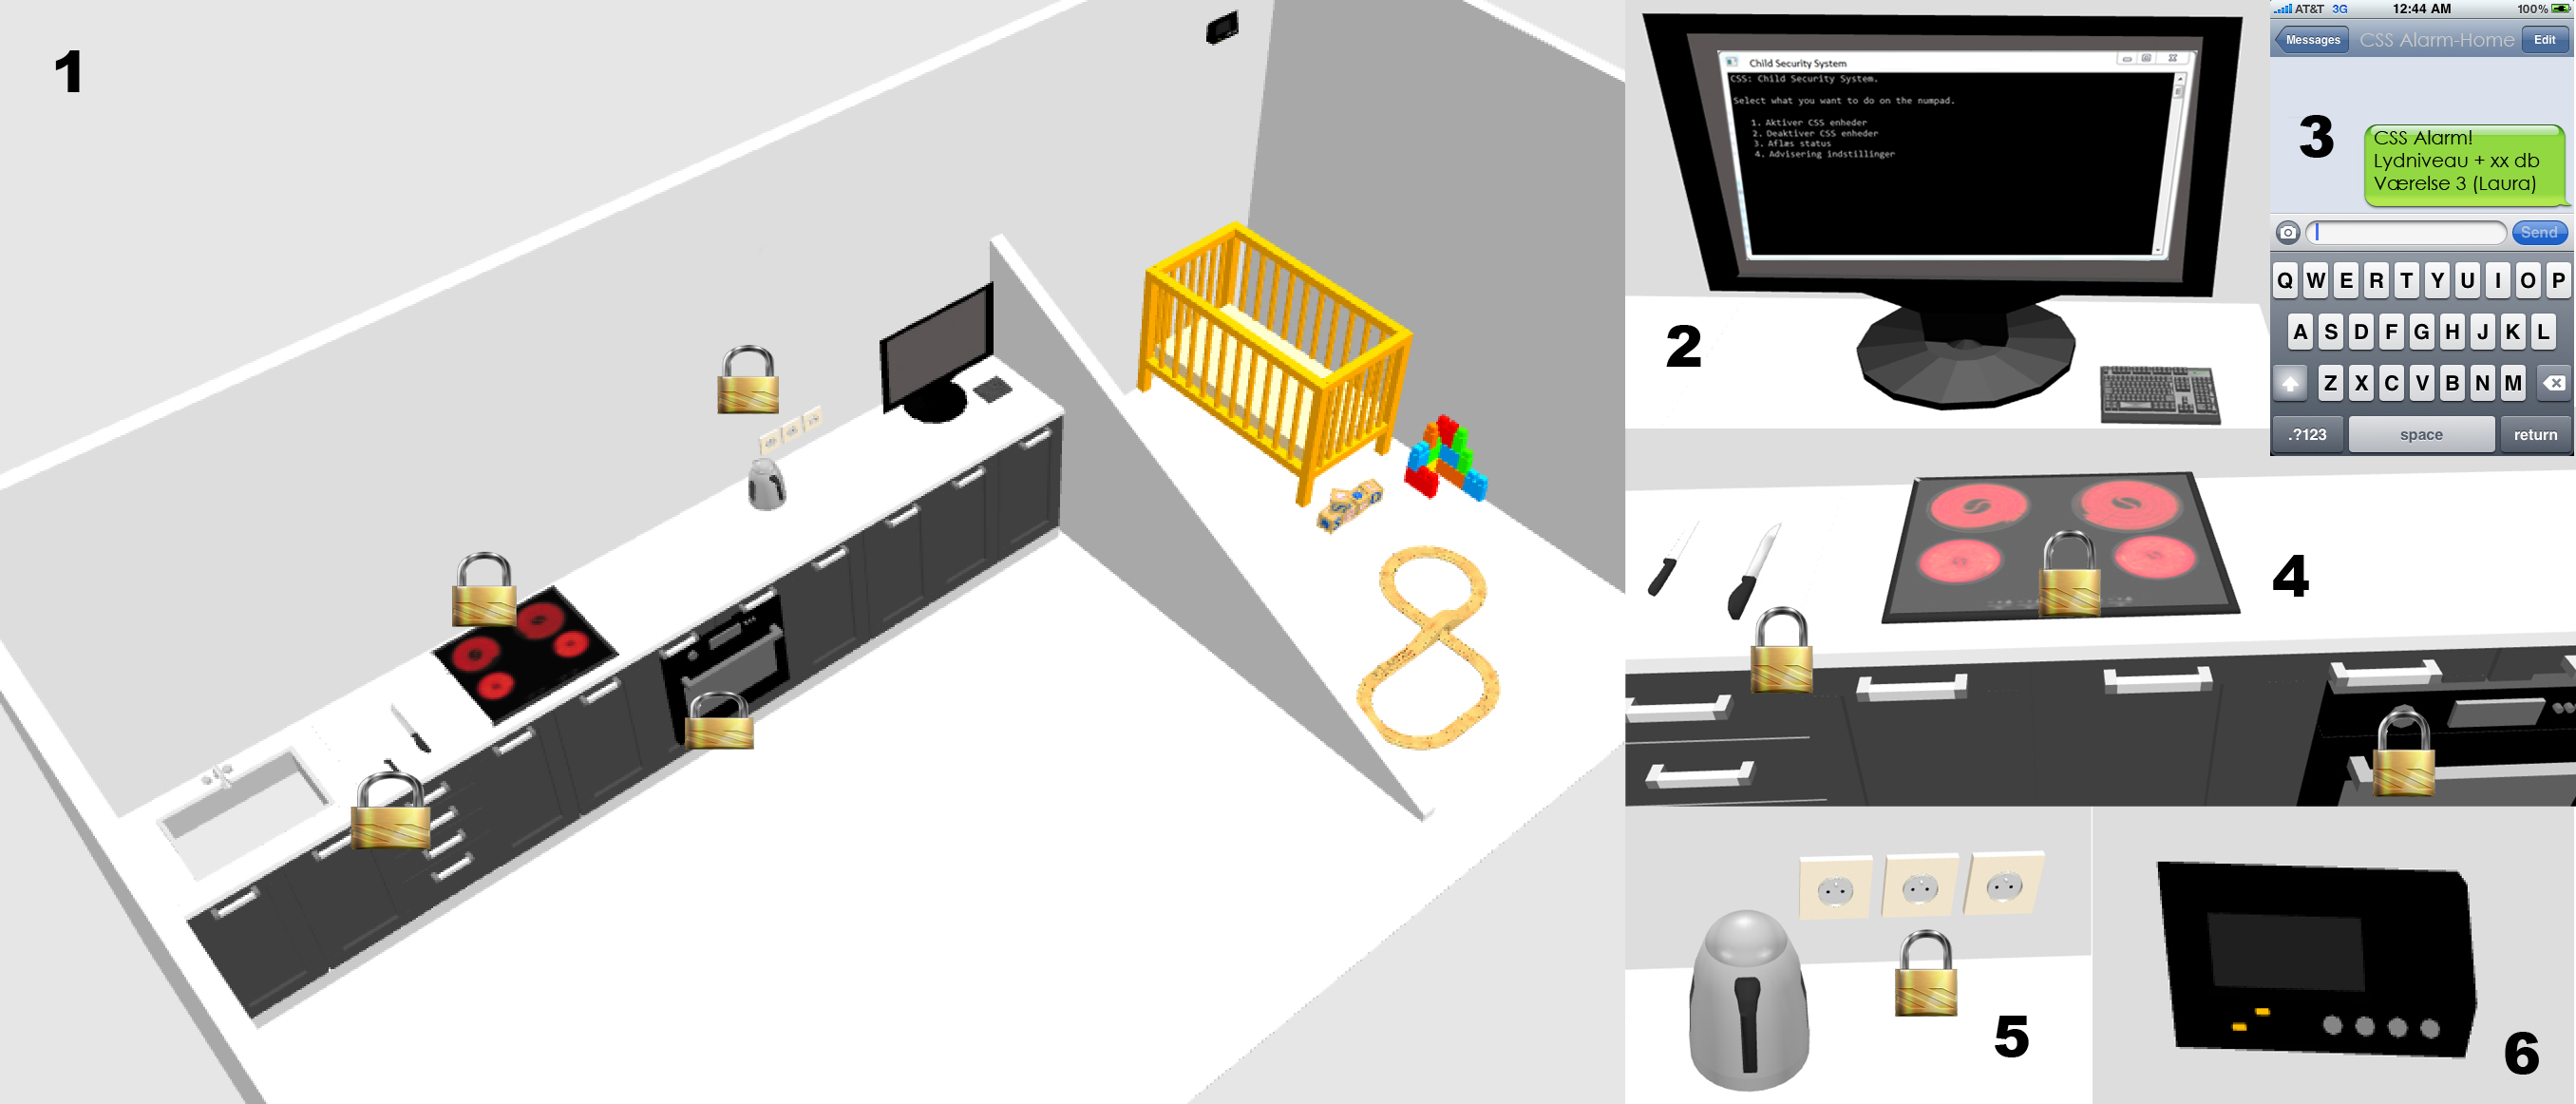
\includegraphics[width=\textwidth]{billeder/Installationsoversigt}}
\caption{Installationsoversigt}
\label{fig:installationsoversigt}
\end{figure}

\begin{enumerate}
\item Samlet oversigtstegning af CSS. 
\item CSS programmet med tilhørende DE2 kodelås
\item SMS besked udsendt af systemet idet lydniveauet i værelse 3 (Laura) har været over det tilladte.
\item Overblik over hvad systemet er tiltænkt at børnesikre. Køkken skuffe med skarpe genstande, kogeplader, ovn.
\item 230V udtag. X10 styret, således at det bestemmes om der udtaget skal være aktivt.
\item Babyalarm. Illustrationen vil variere i forhold til virkeligheden.
\end{enumerate}

\begin{figure}[h] \centering
\fbox{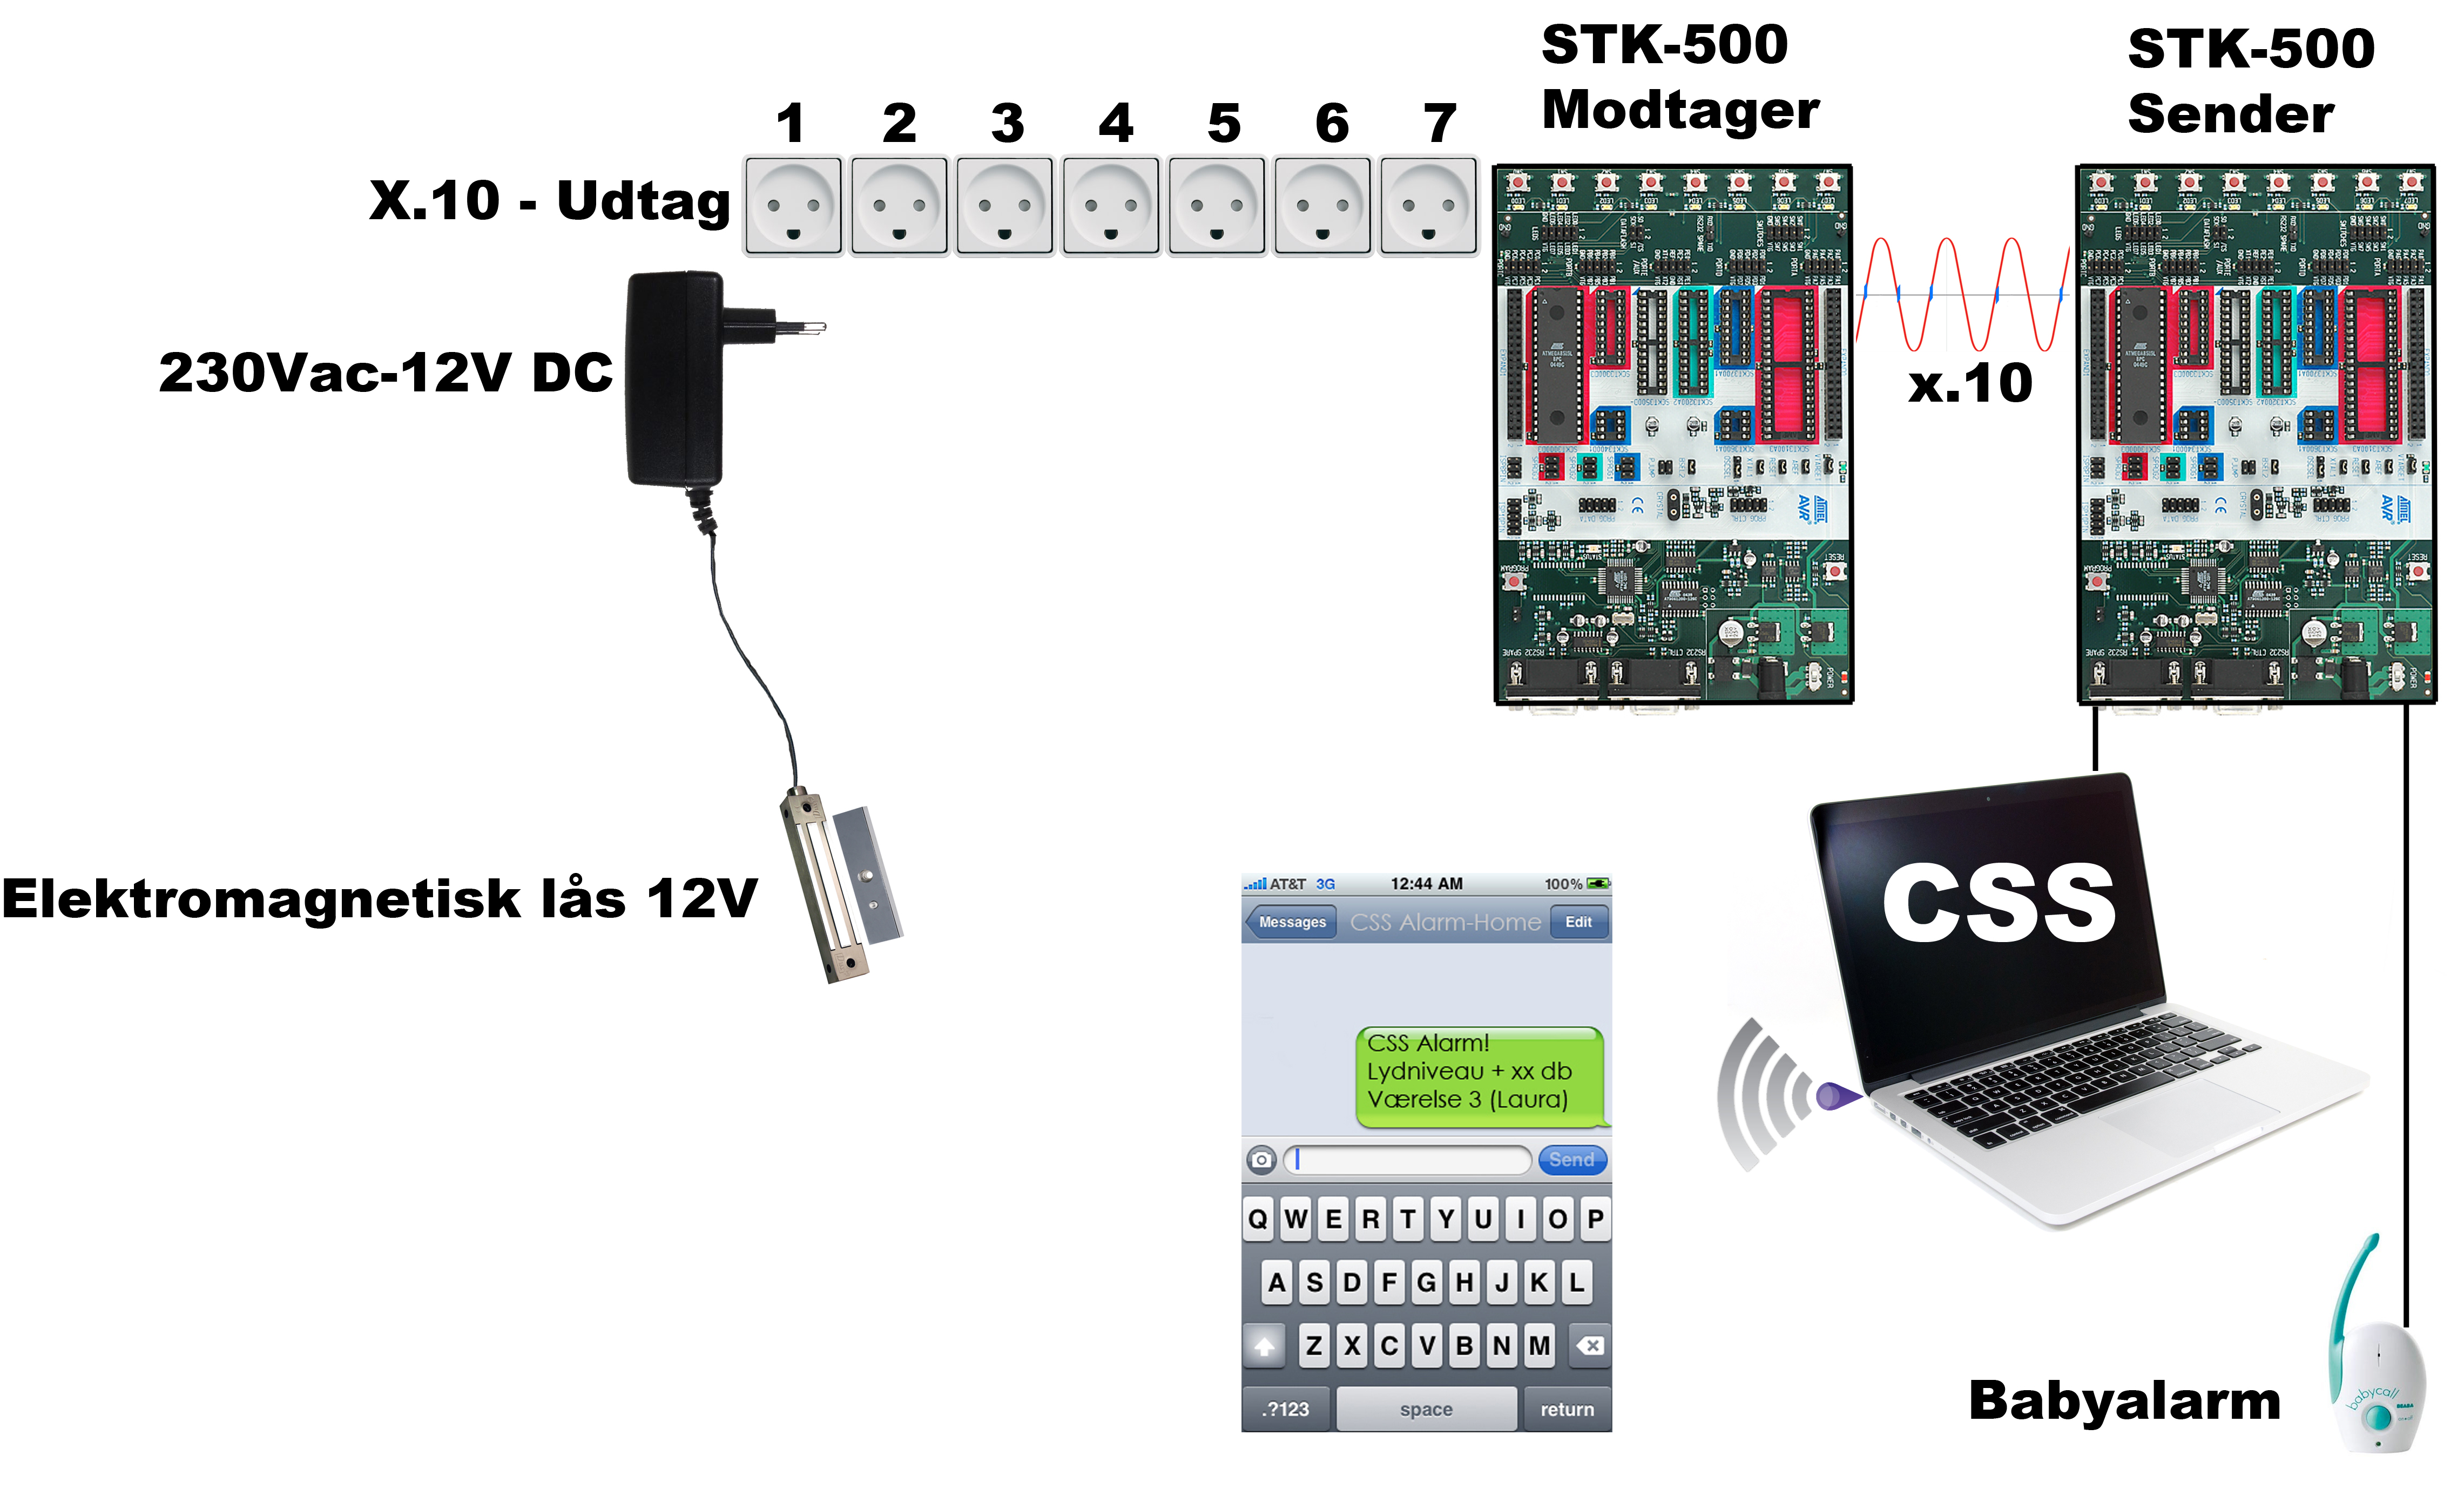
\includegraphics[width=0.65\textwidth]{billeder/Oversigt}}
\caption{Oversigt}
\label{fig:Oversigt}
\end{figure}


Ud fra en kommando fra CSS programmet på computeren styres ønskede 230V udtag i hjemmet. Dette er muligt ved at benytte sig af X10 protokollen. Testmiljøet er illustreret via billedet \ref{lab:Oversigt}. Her sender CSS programmet besked til Hovedenheden som giver Modtageren besked på at hhv. tænde eller slukket for et givent udtag. Hvad brugen tilslutter i de forskellige udtag står frit for. Ydermere er der på X10 senderen koblet en lyddetektor som via computeren sender en sms ud via API.